\subsection{Round 1 Solutions}\label{S::2022-O-1}

\resph{https://www.youtube.com/watch?v=42LFCwMgTwQ}{Review by \textit{Way Tan}}

\begin{question}[4043]\label{A::2022-O-1-1}
    If $S = \displaystyle\sum_{k = -2021}^{2021} \frac{1}{10^k + 1}$, find $\floor{2S}$.
\end{question}

Observe that $\frac{1}{10^{-k} + 1} = \frac{10^k}{10^{k} + 1}$. The $-k$th term can thus be paired with the $k$th term to form $\frac{10^k + 1}{10^k + 1} = 1$, with the $0$th term being the only unpaired term. The sum hence evaluates to \[S = 2021 + \frac{1}{10^0 + 1} \implies \floor{2S} = 4043.\]

\begin{question}[1303]\label{A::2022-O-1-2}
    All the positive integers $1, 2, 3, 4, \cdots,$ are grouped in the following way: $G_1 = \bc{1, 2}$, $G_2 = \bc{3, 4, 5, 6}$, $G_3 = \bc{7, 8, 9, 10, 11, 12, 13, 14}$, that is, the set $G_n$ contains the next $2^n$ positive integers listed in ascending order after the set $G_{n-1}$, $n > 1$. If $S$ is the sum of all the positive integers from $G_1$ to $G_8$, find $\floor{\frac{S}{100}}$.
\end{question}

It is not too hard to show that the last term in $G_n$ is $2^{n+1} - 2$. The last term of $G_8$ is hence $2^9 - 2 = 510$, whence $S$ evaluates to $510(511)/2$. Thus, $\floor{S/100} = 1303$.

\begin{question}[100]\label{A::2022-O-1-3}
    A sequence of one hundred positive integers $x_1, x_2, x_3, \cdots, x_{100}$ are such that \[(x_1)^2 + (2x_2)^2 + (3x_3)^2 + (4x_4)^2 + \cdots + (100x_{100})^2 = 338350.\] Find the largest possible value of $x_1 + x_2 + x_3 + \cdots + x_{100}$.
\end{question}

Observe that $1^2 + 2^2 + 3^2 + \cdots + 100^2 = 338350$. Since $x_i$ are positive integers, they must all be 1 (to prevent the sum from exceeding 338350). The desired value is hence 100.

\clearpage
\begin{question}[9]\label{A::2022-O-1-4}
    Let $a$ and $b$ be two real numbers satisfying $a < b$, and such that for each real number $m$ satisfying $a < m < b$, the circle $x^2 + (y-m)^2 = 25$ meets the parabola $4y = x^2$ at four distinct points in the Cartesian plane. Let $S$ be the maximum possible value of $b-a$. Find $\floor{4S}$.
\end{question}

Note that $a$ is clearly $5$. Now consider the extreme case where $m > 5$ and the circle is tangent to the parabola. The discriminant of the quadratic $4y + (y-m)^2 = 25$ must be 0, whence $m = 29/4$. Hence, $S = b - a = 29/4 - 5 = 9/4$. Thus, $\floor{4S} = 9$.

\begin{question}[11]\label{A::2022-O-1-5}
    Let $P$ be a point within a rectangle $ABCD$ such that $PA = 10$, $PB = 14$ and $PD = 5$, as shown below. Find $\floor{PC}$.
    
    \begin{center}
        \begin{tikzpicture}[scale=0.7]
            \coordinate[label=above left:$A$] (A) at (0, 5);
            \coordinate[label=below left:$B$] (B) at (0, 0);
            \coordinate[label=below right:$C$] (C) at (10, 0);
            \coordinate[label=above right:$D$] (D) at (10, 5);
            \coordinate[label=below right:$P$] (P) at (7, 3);

            \draw (A) -- (B);
            \draw (B) -- (C);
            \draw (C) -- (D);
            \draw (D) -- (A);
            \draw (A) -- (P);
            \draw (D) -- (P);
            \draw (B) -- (P);
        
            \node[anchor=north east] at ($(A)!0.5!(P)$) {10};
            \node[anchor=north west] at ($(D)!0.5!(P)$) {5};
            \node[anchor=north west] at ($(B)!0.5!(P)$) {14};
        \end{tikzpicture}
    \end{center}
\end{question}

By the British flag theorem, one has $10^2 + PC^2 = 5^2 + 14^2$, whence $\floor{PC} = 11$.

\begin{question}[50]\label{A::2022-O-1-6}
    In the diagram below, the rectangle $ABCD$ has area 180 and both triangles $ABE$ and $ADF$ have areas 60. Find the area of triangle $AEF$.

    \begin{center}
        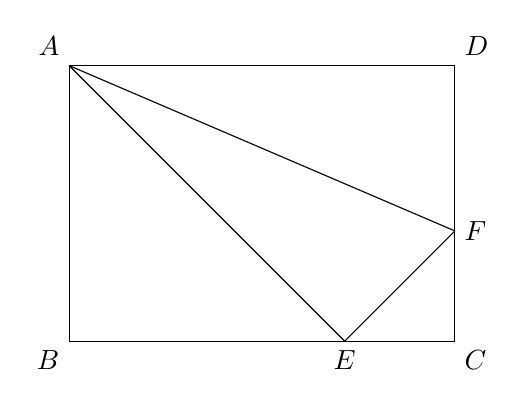
\begin{tikzpicture}[scale=0.7]
            \coordinate[label=above left:$A$] (A) at (0, 5);
            \coordinate[label=below left:$B$] (B) at (0, 0);
            \coordinate[label=below right:$C$] (C) at (7, 0);
            \coordinate[label=above right:$D$] (D) at (7, 5);
            \coordinate[label=below:$E$] (E) at (5, 0);
            \coordinate[label=right:$F$] (F) at (7, 2);

            \draw (A) -- (B);
            \draw (B) -- (C);
            \draw (C) -- (D);
            \draw (D) -- (A);
            \draw (A) -- (E);
            \draw (E) -- (F);
            \draw (A) -- (F);
        \end{tikzpicture}
    \end{center}
\end{question}

Let $BE = x$ and $DF = y$. Observe that $x/(x+EC) = [ABE]/[ABC] = 60/90 = 2/3$. Hence, $EC = x/2$. Similarly, $y/(y+FC) = [ADF]/[ADC] = 60/90 = 2/3$, whence $FC = y/2$. Thus, $[CEF] = [CDE]/3 = [ABE]/6 = 10$. Finally, $[AEF] = 180 - 60 - 60 - 10 = 50$.

\clearpage
\begin{question}[144]\label{A::2022-O-1-7}
    A tetrahedron in $\RR^3$ has one vertex at the origin $O$ and other vertices at the points $A(6, 0, 0)$, $B(4, 2, 4)$ and $C(3, 2, 6)$. If $x$ is the height of the tetrahedron from $O$ to the plane $ABC$, find $\floor{5x^2}$.
\end{question}

The plane $ABC$ is given by the vector equation $\vec r \dotp (2, 0, 1) = 12$. Since $x$ is the perpendicular distance from $O$ to $ABC$, we have $x = 12/{\sqrt{2^2 + 0^2 + 1^2}} = 12/\sqrt5$. Thus, $\floor{5x^2} = 144$.

\begin{question}[208]\label{A::2022-O-1-8}
    Let $x$ and $y$ be real numbers such that $(x-2)^2 + (y-3)^2 = 4$. If $S$ is the largest possible value of $x^2 + y^2$, find $\floor{(S-17)^2}$.
\end{question}

Observe that $(x-2)^2 + (y-3)^2 = 4$ describes a circle with centre $(2, 3)$ and radius 2, while $S$ is the square of the distance from some point $P$ on the circle to the origin. The largest distance clearly occurs when the origin, the centre $(2, 3)$, and $P$ are collinear. This distance can be calculated as $\sqrt{2^2 + 3^2} + 2 = \sqrt{13} + 2$. Hence, \[\floor{(S-17)^2} = \floor{\bp{(\sqrt{13} + 2)^2 - 17}^2} = 208.\]

\begin{question}[18]\label{A::2022-O-1-9}
    Let $S$ be the maximum value of $w^3 - 3w$ subject to the condition that $w^4 + 9 \leq 10w^2$. Find $\floor{S}$.
\end{question}

Consider $w^4 + 9 \leq 10 w^2$. Solving, we have $(w^2 - 9)(w^2 - 1) \leq 0$, whence $w \in [-3, -1] \cup [1, 3]$. Now notice that $w^3 - 3w$ is odd and is increasing when $w < -1$ or $w > 1$. The maximum value thus occurs either at $w = -1$ or $3$. Comparing values, we see that $\floor S = \floor{3^3 - 3\cdot3} = 18$.

\clearpage
\begin{question}[40]\label{A::2022-O-1-10}
    In the quadrilateral $ABCD$ below, it is given that $AB = BC = CD$ and $\angle ABC = 80\deg$ and $\angle BCD = 160 \deg$. Suppose $\angle ADC = x\deg$. Find the value of $x$.

    \begin{center}
        \begin{tikzpicture}[scale=0.7]
            \coordinate[label=left:$A$] (A) at (0, 0);
            \coordinate[label=left:$B$] (B) at (0.7, 3);
            \coordinate[label=right:$C$] (C) at (3.5, 2.5);
            \coordinate[label=right:$D$] (D) at (5, 0);

            \draw (A) -- (B);
            \draw (B) -- (C);
            \draw (C) -- (D);
            \draw (D) -- (A);
        \end{tikzpicture}
    \end{center}
\end{question}

\begin{center}
    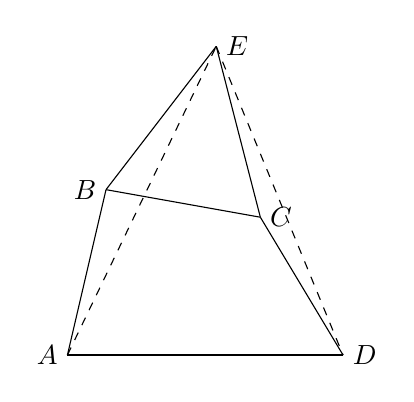
\begin{tikzpicture}[scale=0.7]
        \coordinate[label=left:$A$] (A) at (0, 0);
        \coordinate[label=left:$B$] (B) at (0.7, 3);
        \coordinate[label=right:$C$] (C) at (3.5, 2.5);
        \coordinate[label=right:$D$] (D) at (5, 0);
        \coordinate[label=right:$E$] (E) at (2.7, 5.6);

        \draw (A) -- (B);
        \draw (B) -- (C);
        \draw (C) -- (D);
        \draw (D) -- (A);
        \draw (B) -- (E);
        \draw (C) -- (E);
        \draw[dashed] (A) -- (E);
        \draw[dashed] (E) -- (D);

        \tkzMarkSegment[pos=.5,mark=|](A,B);
        \tkzMarkSegment[pos=.5,mark=|](B,E);
        \tkzMarkSegment[pos=.5,mark=|](C,E);
        \tkzMarkSegment[pos=.5,mark=|](C,D);
        \tkzMarkSegment[pos=.5,mark=|](C,B);
    \end{tikzpicture}
\end{center}

Let $E$ be such that $\triangle BCE$ is equilateral, as shown above.

Note that $\triangle ABE$ is isosceles. Since $\angle ABE = 80\deg + 60 \deg = 140 \deg$, we have $\angle BAE = \angle BEA = 20\deg$. Hence, $\angle AED = 60\deg - 20\deg = 40\deg$. However, notice that $\triangle DCE$ is also isosceles, and reflex $\angle CDE = 360\deg - 60\deg - 160\deg = 140\deg$. Thus, $\angle CED = \angle CDE = 20 \deg$, whence $\triangle ABE \equiv \triangle DCE$, implying $AE = DE$. Because $\angle AED = 40\deg + 20\deg = 60\deg$, it follows that $\triangle AED$ is equilateral, thus giving $x\deg = 60\deg - 20\deg = 40\deg$. 

\begin{question}[544]\label{A::2022-O-1-11}
    Let $a$, $b$, $c$ be integers with $ab + c = 49$ and $a + bc = 50$. Find the largest possible value of $abc$.
\end{question}

Subtracting the two equations, we obtain $a + bc - ab - c = 1$. This can be factorized as $(b-1)(c-a) = 1$. Since $a$, $b$ and $c$ are integers, we are left with two cases:

\case{1}[$b-1 = c-a = -1$] We have $b = 0$, whence $abc = 0$.

\case{2}[$b-1 = c-a = 1$] We have $b = 2$ and $c = 1 + a$. Substituting this back into one of the original equations, we get $a = 16$ and $c = 17$, whence $abc = 544$.

The largest possible value of $abc$ is thus 544.

\begin{question}[17]\label{A::2022-O-1-12}
    Find the largest possible value of $\abs a + \abs b$, where $a$ and $b$ are coprime integers (i.e., $a$ and $b$ are integers which have no common factors larger than 1) such that $\frac{a}{b}$ is a solution of the equation below: \[\sqrt{4x + 5 - 4\sqrt{x+1}} + \sqrt{x+2 - 2\sqrt{x+1}} = 1.\]
\end{question}

Note that \[4x + 5 - 4\sqrt{x+1} = \bp{2\sqrt{x+1}}^2 - 2\cdot\sqrt{x+1}\cdot1 + 1^2 = \bp{2\sqrt{x+1} - 1}^2\] and \[x + 2 - 2\sqrt{x+1} = \bp{\sqrt{x+1}}^2 - 2\cdot\sqrt{x+1}\cdot 1 + 1^2 = \bp{\sqrt{x+1} - 1}^2.\] We hence have \[\pm \bp{2\sqrt{x+1} - 1} \pm \bp{\sqrt{x+1} - 1} = 1.\]

\case{1}[$\bp{2\sqrt{x+1} - 1} + \bp{\sqrt{x+1} - 1} = 1$] We have $3\sqrt{x+1} = 3$, whence $x = 0$. Hence, $a = 0$ and $b = 1$, whence $\abs a + \abs b = 1$.

\case{2}[$\bp{2\sqrt{x+1} - 1} - \bp{\sqrt{x+1} - 1} = 1$] We have $\sqrt{x+1} = 3$, whence $x = 8$. Hence, $a = 8$ and $b = 1$, whence $\abs a + \abs b = 9$.

\case{3}[$-\bp{2\sqrt{x+1} - 1} + \bp{\sqrt{x+1} - 1} = 1$] We have $\sqrt{x+1} = -1$, a contradiction.

\case{4}[$-\bp{2\sqrt{x+1} - 1} - \bp{\sqrt{x+1} - 1} = 1$] We have $3\sqrt{x+1} = 1$, whence $x = -8/9$. Hence, $a = -8$ and $b = 9$, whence $\abs a + \abs b = 17$.

The maximum value of $\abs a + \abs b$ is 17.

\begin{question}[3000]\label{A::2022-O-1-13}
    Let $S$ be the set of real solutions $(x, y, z)$ of the following system of equations: \[\left\{
        \begin{aligned}
            \frac{4x^2}{1 + 4x^2} = y,\\
            \frac{4y^2}{1 + 4y^2} = z,\\
            \frac{4z^2}{1 + 4z^2} = x.
        \end{aligned}\right.\] For each $(x, y, z) \in S$, define $m(x, y, z) = 2000(\abs x + \abs y + \abs z)$. Determine the maximum value of $m(x, y, z)$ over all $(x, y, z) \in S$.
\end{question}

Taking reciprocals, we have \[\left\{
    \begin{aligned}
        1 + \frac1{4x^2} = \frac1y,\\
        1 + \frac1{4y^2} = \frac1z,\\
        1 + \frac1{4z^2} = \frac1x.
\end{aligned}\right.\] Summing, we obtain \[\bs{\dfrac1{(2x)^2} - \dfrac1x + 1} + \bs{\dfrac1{(2y)^2} - \dfrac1y + 1} + \bs{\dfrac1{(2z)^2} - \dfrac1z + 1} = 0.\] This clearly factors as \[\bp{\dfrac1{2x} - 1}^2 + \bp{\dfrac1{2y} - 1}^2 + \bp{\dfrac1{2z} - 1}^2 = 0,\] whence $x = y = z = 1/2$, giving $\max m(x, y, z) = 3000$.

\clearpage
\begin{question}[11]\label{A::2022-O-1-14}
    Assume that $t$ is a positive solution to the equation \[t = \sqrt{1 + \sqrt{1 + \sqrt{1 + \sqrt{1 + t}}}}.\] Determine the value of $t^4 - t^3 - t + 10$.
\end{question}

Observe that $t = \sqrt{1 + t}$. It follows that $t^2 - t - 1 = 0$, whence $t$ is the golden ratio $\vf$, which has the property that $\vf^n = \vf^{n-1} + \vf^{n-2}$ for all integers $n$. The desired value is hence \[t^4 - t^3 - t + 10 = t^2 - t + 10 = 1 + 10 = 11.\]

\begin{question}[44]\label{A::2022-O-1-15}
    In the triangle $ABC$ shown in the diagram below, the external angle bisectors of $\angle B$ and $\angle C$ meet at the point $D$. The tangent from $D$ to the incircle $\o$ of the triangle $ABC$ touches $\o$ at $E$, where $E$ and $B$ are on the same side of the line $AD$. Suppose $\angle BEC = 112\deg$. Find the size of $\angle A$ in degrees.

    \begin{center}
        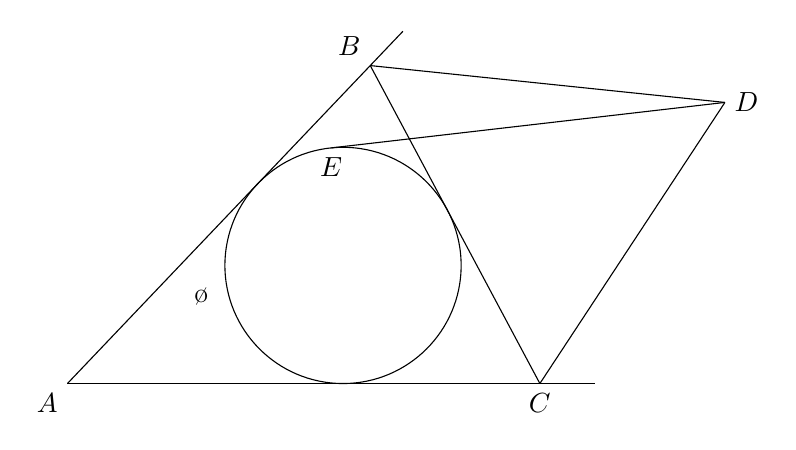
\begin{tikzpicture}
            \coordinate[label=below left:$A$] (A) at (0, 0);
            \coordinate[label=above left:$B$] (B) at (3.846, 4.038);
            \coordinate[label=below:$C$] (C) at (6, 0);
            \coordinate[label=right:$D$] (D) at (8.35, 3.57);
            \coordinate[label=below:$E$] (E) at (3.34871, 2.9923);

            \draw (3.5, 1.5) circle[radius=1.5];

            \draw (A) -- (4.26, 4.473);
            \draw (B) -- (C);
            \draw (6.7, 0) -- (A);
            
            \draw (D) -- (E);
            \draw (B) -- (D);
            \draw (C) -- (D);

            \node at (1.7, 1.1) {$\o$};
        \end{tikzpicture}
    \end{center}
\end{question}

\begin{center}
    \begin{tikzpicture}
        \coordinate[label=below left:$A$] (A) at (0, 0);
        \coordinate[label=above left:$B$] (B) at (3.846, 4.038);
        \coordinate[label=below:$C$] (C) at (6, 0);
        \coordinate[label=right:$D$] (D) at (8.35, 3.57);
        \coordinate[label=below left:$E$] (E) at (3.34871, 2.9923);
        \coordinate[label=below:$I$] (I) at (3.5, 1.5);

        \draw (I) circle[radius=1.5];

        \draw (A) -- (4.26, 4.473);
        \draw (B) -- (C);
        \draw (6.7, 0) -- (A);
        
        \draw (D) -- (E);
        \draw (B) -- (D);
        \draw (C) -- (D);

        \node at (1.7, 1.1) {$\o$};

        \fill (I) circle[radius=1pt];

        \draw[dashed] (B) -- (I);
        \draw[dashed] (C) -- (I);
        \draw[dashed] (E) -- (I);
        \draw[dashed] (I) -- (D);

        \draw pic [draw, angle radius=2mm, ""] {right angle = D--E--I};
        \draw pic [draw, angle radius=2mm, ""] {right angle = D--B--I};
        \draw pic [draw, angle radius=2mm, ""] {right angle = D--C--I};

    \end{tikzpicture}
\end{center}

Let $I$ be the incentre of $\triangle ABC$. Observe that $BI$ and $IC$ bisect $\angle B$ and $\angle C$ respectively. Hence, $\angle IBD = \angle ICD = 90\deg$. Furthermore, since $ED$ is tangent to $\o$, we have $\angle IED = 90\deg$. Thus, $B$, $C$, $D$, $E$ and $I$ are concyclic, with $ID$ as the diameter. Hence, $\angle BIC = \angle BEC = 112\deg$. Since $IB$ and $IC$ are angle bisectors, we have \[\angle B + \angle C = 2 \bp{\angle IBC + \angle ICB} = 2 \bp{180\deg - 112\deg} = 136\deg.\] It immediately follows that $\angle A = 180\deg - 136\deg = 44\deg$.

\begin{question}[99]\label{A::2022-O-1-16}
    Find the largest integer $n$ such that $n^2 + 5n - 9486 = 10s(n)$, where $s(n)$ is the product of all digits of $n$ in the decimal representation of $n$.
    
    \noindent (For example, $s(481) = 4 \times 8 \times 1 = 32.$)
\end{question}

Observe that $s(n) \leq n$ for all $n$. We thus have the inequality $n^2 + 5n - 9486 \leq 10 n$, whence it is clear that the largest possible $n$ is 99.

\begin{question}[8]\label{A::2022-O-1-17}
    Find the number of integer solutions to the equation $19x + 93y = 4xy$.
\end{question}

Note that $(ax+b)(cy+d) = adx + acxy + bcy + bd$, where $a$, $b$, $c$ and $d$ are real numbers. Comparing this to the given equation, we have $ad = 19$, $ac = -4$ and $bc = 93$. Taking $a = 1$, $c = -4$, $b = -93/4$ and $d = 19$, we have \[\bp{x - \frac{93}{4}}(-4y + 19) = -\dfrac{19 \cdot 93}{4}.\] Upon simplification, one gets \[(4x - 93)(4y-19) = -1 \cdot 3 \cdot 19 \cdot 31.\] Observe that both $4x - 93$ and $19 - 4y$ are congruent to 1 modulo 4. On the other hand, all four factors ($-1$, 3, 19 and 31) are also congruent to 3 modulo 4. We must hence have an even number of factors contributing to both terms. This narrows the possibilities down to a few cases.

\case{1}[Both terms have two factors] The number of possibilities in this case is $\comb{4}{2} = 6$.

\case{2}[One term has four factors, the other has none] The number of possibilities in this case is clearly 2.

Altogether, there are $6 + 2 = 8$ possibilities, thus there are 8 integer solutions to the given equation.

\begin{question}[121]\label{A::2022-O-1-18}
    Find the number of integer solutions to the equation $x_1 + x_2 - x_3 = 20$ with $x_1 \geq x_2 \geq x_3 \geq 0$.
\end{question}

Rewriting the equation, we have $x_1 + x_2 = 20 + x_3$. Suppose $x_3$ is fixed (and admits possible values of $x_2$ and $x_1$). Observe that $x_1 \leq 20$, with equality only when $x_2 = x_3$. The only possible values of $x_1$ are hence $\bc{20, 19, 18, \cdots, x_2}$. However, since $x_1 \geq x_2$, we have the condition $x_2 \leq \floor{\frac12 (20 + x_3)}$. The number of solutions for a given $x_3$ is hence $11 - \floor{\frac12 x_3}$. The total number of integer solutions is thus \[11 + 10 + 10 + 9 + 9 + \cdots + 1 + 1 = 11 + 2 \cdot \frac{10 \cdot 11}{2} = 121.\]

\clearpage
\begin{question}[2]\label{A::2022-O-1-19}
    In the diagram below, $E$ is a point outside a square $ABCD$ such that $CE$ is parallel to $BD$, $BE = BD$, and $BE$ intersects $CD$ at $H$. Given $BE = \sqrt6 + \sqrt2$, find the length of $DH$.

    \begin{center}
        \begin{tikzpicture}[scale=0.6]
            \coordinate[label=above left:$A$] (A) at (0, 5);
            \coordinate[label=below left:$B$] (B) at (0, 0);
            \coordinate[label=below right:$C$] (C) at (5, 0);
            \coordinate[label=above right:$D$] (D) at (5, 5);
            \coordinate[label=right:$E$] (E) at (6.83, 1.83);
            \coordinate[label=above left:$H$] (H) at (5, 1.34);
            
            \draw (A) -- (B);
            \draw (B) -- (C);
            \draw (C) -- (D);
            \draw (D) -- (A);
            \draw[->-=0.5] (B) -- (D);
            \draw (B) -- (E);
            \draw[->-=0.5] (C) -- (E);
        \end{tikzpicture}
    \end{center}
\end{question}

\sol{1} Observe that $\triangle HDB$ is similar to $\triangle HCE$. Hence, \[\frac{EH}{BH} = \frac{CH}{DH} \implies \frac{BE-BH}{BH} = \frac{DC-DH}{DH} \implies \frac{BE}{BH} = \frac{DC}{DH}.\] Note that the side length of the square is $\frac1{\sqrt2} BD = \sqrt3 + 1$. Thus, \[\frac{\sqrt6 + \sqrt2}{BH} = \frac{\sqrt3 + 1}{DH} \implies BH^2 = 2DH^2.\] Using Pythagoras' theorem on $\triangle BCH$, one obtains \[BC^2 + CH^2 = BH^2 \implies \bp{\sqrt3 + 1}^2 + \bp{\sqrt3 + 1 - DH}^2 = 2DH^2.\] Solving, we have $DH = 2$.

\sol{2}[Abusing integers] Note that the side length of the square is $\frac1{\sqrt2} BD = \sqrt3 + 1 \approx 2.73$. Since $DH$ is an integer and $CH < DH < BD$, it must be 2.

\begin{question}[4]\label{A::2022-O-1-20}
    The diagram below shows the region $R = \bc{(x, y) \in \RR^2 | y \geq \frac12 x^2}$ on the $xy$-plane bounded by the parabola $y = \frac12 x^2$. Let $C_1$ be the largest circle lying inside $R$ with its lowest point at the origin. Let $C_2$ be the largest circle lying inside $R$ and resting on top of $C_1$. Find the sum of radii of $C_1$ and $C_2$.
    
    \begin{center}
        \begin{tikzpicture}[scale=0.7]
            \begin{axis}[
                domain = -5:5,
                ymax=8,
                axis line style={draw=none},
                tick style={draw=none},
                xticklabel = \empty,
                yticklabel = \empty,
                ]
                \addplot[black] {0.5 * x^2};
    
                \draw (0, 1) circle[radius=1];
                \draw (0, 5) circle[radius=3];
            \end{axis}
        \end{tikzpicture}
    \end{center}
\end{question}

Let the radius of $C_1$ and $C_2$ be $r_1$ and $r_2$ respectively. The equations of $C_1$ and $C_2$ are hence
\begin{align*}
    C_1 &: x^2 + (y-r_1)^2 = r_1^2,\\
    C_2 &: x^2 + (y-(2r_1+r_2))^2 = r_2^2.
\end{align*}

Consider the intersection between $C_1$ and the parabola: \[\left\{
    \begin{aligned}
        y &= \frac12 x^2\\
        x^2 + (y-r_1)^2 &= r_1^2
    \end{aligned}
\right.\] This gives $y^2 + 2y(1 - r_1) = 0$. Since the two curves only intersect at the origin, we have $r_1 = 1$.

Now consider the intersection between $C_2$ and the parabola: \[\left\{
    \begin{aligned}
        y &= \frac12 x^2\\
        x^2 + (y-(2r_1+r_2))^2 &= r_2^2
    \end{aligned}
\right.\] This gives $y^2 - 2y(1 + r_2) + 4(1 + r_2) = 0$. By symmetry, the two curves intersect at a unique $y$-value, hence the discriminant is 0. We hence obtain $4(1+r_2)^2 - 16(1+r_2) = 0$, whence $r_2 = 3$. The required sum is thus $1 + 3 = 4$.

\begin{question}[30]\label{A::2022-O-1-21}
    Find the smallest positive integer $x$ such that $3x^2 + x = 4y^2 + y$ for some positive integer $y$.
\end{question}

Completing the square, one gets \[4(6x+1)^2 - 4 = 3(8y+1)^2 - 3\] after simplification. This can be rewritten as \[(12x+2)^2 - 3(8y+1)^2 = 1,\] which one may recognize as a case of Pell's equation. We hence consider the equation $X^2 - 3Y^2 = 1$. The fundamental solution is clearly $X = 2$ and $Y = 1$. We now have the following standard recurrence relations for $X$ and $Y$: \[X_{k+1} = 2X_k + 3Y_k, \quad Y_{k+1} = 2Y_k + X_k.\] Keeping in mind that $X$ is of the form $12x + 2$ and $Y$ is of the form $8y +1$, the first valid solution occurs when $k = 5$, where $X = 362$ and $Y = 209$, which corresponds to $x = 30$ and $y = 26$.

\begin{question}[200]\label{A::2022-O-1-22}
    A group of students participates in some sports activities among 6 different types of sports. It is known that for each sport activity there are exactly 100 students in the group participating in it; and the union of all the sports activities participated by any two students is NOT the entire set of 6 sports activities. Determine the minimum number of students in the group.
\end{question}

Let $m$ be the maximum number of sports a student can take at once. By symmetry, we only need to consider $m \geq 3$ (any $m < 3$ will lead to a less-than-optimal allocation of students). Furthermore, it is obvious that $m \geq 5$ is impossible, since it would immediately violate the given restriction. We hence analyse only the $m = 3$ and $m = 4$ case.

\case{1}[$m = 4$] To adhere to the given restriction, there is only one possible allocation of students: 100 to Sport A, 100 to Sport B and 100 taking the other four sports. This gives a total of 300 students.

\case{2}[$m = 3$] Note that the absolute minimum number of students is given by $100 \cdot 6 / 3 = 200$. We now construct an allocation that uses exactly 200 students.

Let the sports be labelled A through F. Consider the following allocation of students:
\begin{table}[H]
    \centering
    \begin{tabular}{|l|l|l|l|l|l|l|}
    \hline
     & A & B & C & D & E & F \\ \hline
    Student 1 & X & X & X &  &  &  \\ \hline
    Student 2 & X &  &  & X & X &  \\ \hline
    Student 3 &  & X &  & X &  & X \\ \hline
    Student 4 &  &  & X &  & X & X \\ \hline
    \end{tabular}
\end{table}
Repeating the above allocation 50 times, we will have 100 students per sport. Hence, the minimum number of students is $4 \cdot 50 = 200$ as desired.

\begin{question}[29]\label{A::2022-O-1-23}
    Let $p$ and $q$ be positive prime integers such that $p^3 - 5p^2 - 18p = q^9 - 7q$. Determine the smallest value of $p$.
\end{question}

Observe that the RHS will grow incredibly fast as compared to the LHS. We hence test small values of $q$. Comparing leading terms, we also note that $p \approx q^3$. Furthermore, we require $p^3 - 5p^2 - 18p > 0$, whence $p \geq 11$.

\case{1}[$q = 2$] We have $p\bp{p^2 - 5p - 18} = 2 \cdot 3 \cdot 83$. It can be easily shown that there are no solutions in this case.

\case{2}[$q = 3$] We have $p\bp{p^2 - 5p - 18} = 2 \cdot 3 \cdot 29 \cdot 113$. Testing $p = 29$, we see that it is indeed a solution.

Hence, the smallest value of $p$ is 29.

\begin{question}[27648]\label{A::2022-O-1-24}
    Given that $a$, $b$, $c$ are positive real numbers such that $a + b + c = 9$, find the maximum value of $a^2 b^3 c^4$.
\end{question}

Note that \[9 = a + b + c = \frac{a}{2} + \frac{a}{2} + \frac{b}{3} + \frac{b}{3} + \frac{b}{3} + \frac{c}{4} + \frac{c}{4} + \frac{c}{4} + \frac{c}{4}.\] By the Cauchy-Schwarz inequality, we obtain \[\frac19 \cdot 9 \geq \sqrt[9]{\frac{a^2 b^3 c^4}{2^2 3^3 4^4}}.\] Hence, the maximum value of $a^2 b^3 c^4$ is $2^2 3^3 4^4 = 27648$.

\begin{question}[2023]\label{A::2022-O-1-25}
    Let $\RR^+$ be the set of all positive real numbers. Let $f : \RR^+ \to \RR^+$ be a function satisfying \[xy f(x) \big(f(y) - f(yf(x))\big) = 1\] for all $x, y \in \RR^+$. Find $f(\frac1{2022})$.
\end{question}

Letting $y = 1$, we get the following expression for $f^2(x)$: \[f^2(x) = f(1) - \frac{1}{xf(x)}. \tag{1}\] Replacing $y$ with $f(y)$ in the original equation gives \[f^2(y) = \frac{1}{xf(y)f(x)} + f(f(y)f(x)). \tag{2}\] Substituting (1) into (2) yields \[f(1) - \frac{1}{yf(y)} = \frac{1}{xf(y)f(x)} + f(f(y)f(x)). \tag{3}\] Swapping $x$ and $y$ gives a similar equation: \[f(1) - \frac{1}{xf(x)} = \frac{1}{yf(x)f(y)} + f(f(x)f(y)).\tag{4}\] Subtracting (4) from (3) and simplifying, we obtain \[yf(y) - y = xf(x) - x,\] from which it is clear that for all $x \in \RR^+$, we have $xf(x) - x = c$ for some constant $c$. This immediately gives $f(x) = 1 + \frac{c}{x}$. Substituting this into (1), we have \[1 + \frac{c}{1 + \frac{c}{x}} = \bp{1 + \frac{c}{1}} - \frac{1}{x \bp{1 + \frac{c}{x}}},\] whence $c^2 = 1$. Since the range of $f$ is $\RR^+$, we take $c = 1$, thus $f(x) = 1 + \frac1{x}$ and $f(\frac{1}{2022}) = 2023$.